\documentclass[notitlepage,12pt]{report}
\usepackage[left=0.5in, right=0.5in, top=0.5in, bottom=0.65in]{geometry}

\usepackage{titling}
\usepackage{lipsum}
\usepackage{braket}
\usepackage{graphicx}
\usepackage[table]{xcolor}
\graphicspath{./images/}
\usepackage{subcaption}
\newcommand{\tr}{\mathrm{tr}}
\usepackage{hyperref}
\usepackage{authblk}
\usepackage[backend=biber, style=chem-acs]{biblatex}
\usepackage{tabularx}
% \usepackage{amsmath}
\usepackage{mathtools}% Loads amsmath
\usepackage{physics}
\usepackage{wrapfig}
\renewcommand\thesection{\arabic{section}}

\bibliography{bib}
\addbibresource{bib.bib}

\def\br{{\mathbf{r}}}
\def\bG{{\mathbf{G}}}
\def\brp{{\mathbf{r}^\prime}}


\begin{document}
\renewcommand\Affilfont{\itshape\small}
\begin{center}
    \textbf{\LARGE Accurate models of molecular bulk systems from first principles}\\
    Jessica Martinez, Rutgers University-Newark
\end{center}

\textbf{\large 1.\ Motivations and scientific basis for the collaboration}

    The Pavanello and Gomes groups develop electronic structure methods for the in-silico prediction of molecular and materials properties. The two groups have been collaborating since 2014 and the collaboration so far produced one journal article \supercite{tolle2019charged} and resulted in training of 3 Rutgers-based PhD students and the development of three software modules in the softwares: the subsystem DFT code eDFTpy\supercite{edftpy} based on Quantum ESPRESSO \supercite{qe}, DIRAC \supercite{saue2020dirac}, and other scripting frameworks for quantum chemical simulations, such as PyADF \supercite{Jacob_2011} and Psi4Numpy \supercite{smith2018psi4numpy}. The collaboration has been fuelled by two visits of Prof Gomes to Rutgers in 2014 and 2016. Unfortunately, the past two years have been negatively affected by the COVID pandemic and any international travel was forbidden. 

    Since joining Rutgers as a PhD student in 2019, I have been working on applying the methods developed by the collaboration to determine the ionization potential of liquid water and dissect its dependence on order parameters of the liquid (e.g., the instantaneous structure of  the liquid surrounding a particular molecule that is being ionized).   With the Chateaubriand fellowship, I will be able to travel to Prof Gomes's lab and not only extend the currently available computational method  but also to implement completely new electronic structure methods. I will then apply the resulting software to shed light on timely and important questions related to the electron and nuclear dynamics following an ionization or an X-Ray absorption in condensed phases. Such questions are particularly timely given the several novel experimental techniques based on facility-based free electron lasers that probe electron dynamics at the attosecond timescale \supercite{Duris_2019}.  

    The accurate description of processes occurring in condensed-phase molecular systems requires a symbiotic  equilibrium between spectroscopic techniques\supercite{reimann2021two,malerz2021low,bolognesi2021combined} and computational approaches \supercite{couto2007understanding,ambrosio2016structural,ozaki2021advances}. For example, photoelectron spectroscopy \supercite{thurmer2021accurate,perry2020ionization,credidio2021quantitative,thurmer2021valence,tolle2019charged,gaiduk2018electron,gaiduk2016photoelectron,seidel2016valence} and X-Ray absorption spectroscopy (XAS)\supercite{zhovtobriukh2019liquid,zhang2020isotope,smith2020femtosecond} are among those experimental characterization techniques that routinely rely on computational methods for the resolution of the spectra or their interpretation.
	
    In-depth knowledge of the factors influencing, e.g., the ionization potential (IP) of liquid water could allow the control and better understanding of many crucial processes in electrochemistry\supercite{marenich2014computational}, photochemistry\supercite{reuther1996primary,hu2021photochemical} as well as peculiar states of matter like excess electrons solvated in liquid water\supercite{ambrosio2017electronic}.  Recent advances in liquid microjet  photoelectron spectroscopy have opened the door to the determination of accurate electronic energetics of water and aqueous solutions \supercite{thurmer2021accurate,perry2020ionization,credidio2021quantitative,thurmer2021valence} deliverng the  most accurate value for the IP of liquid water, 11.33 $\pm$0.03 eV.  Such advances have, in turn, prompted simulations to provide an equally accurate description of ionization using electronic structure techniques, such as GW based on periodic pseudopotential DFT \supercite{gaiduk2018electron,ziaei2018probing,dal2014pseudopotentials} delivering excellent agreement with the experiment.
	
    Along similar lines of research, the {\bf Pavanello and Gomes groups} recently developed a method which we call ``impurity model'' based on subsystem DFT \supercite{jacob2014subsystem,wesolowski2015frozen,krishtal2015subsystem} for computing ionization energies (both electron attachment and detachment) of bulk molecular systems \supercite{tolle2019charged}. In subsystem DFT,  the total electron density, $\rho(\br)$ is divided into a sum of subsystem densities 
\begin{equation}
    \label{dens}
    \rho(\br) = \sum_I^{N_S}\rho_I(\br)
\end{equation}
    where $N_S$ is the number of independent subsystems in the simulation and the subsystems are identified by each non-covalently bonded molecule constituting the condensed phase. The subsystem electron densities are determined by a variational procedure which imposes the total energy functional to be stationary wrt variations of each subsystem density. The core of the impurity model is that a $\Delta$SCF procedure\supercite{bagus1965self,waskom2017mwaskom} can be used to compute ionization energies, for the IP we use $IP=E^+-E^0$ where $E^{+/0}$ is the total energy of the ionized/neutral system. The main issue arises when employing periodic boundary conditions (which is the most common method for approaching bulk systems with atomistic models) because a charged system has an infinite energy due to the self-interaction of the excess charge between the infinite number of periodic images. The impurity model solves this problem by subdividing the subsystems into two categories: (1) finite subsystems, whose Coulomb potential is given by the nonperiodic potential (i.e., $v[\rho^{\text{finite}}](\br)=\int\frac{\rho^{\text{finite}}(\brp)}{|\brp-\br|}d\brp$); (2) extended subsystems, whose potential is given by the fully periodic one (i.e., in reciprocal space, $\tilde v[\rho^{\text{extended}}](\bG)=\frac{4\pi}{|\bG|^2}\tilde\rho^\text{extended}(\bG)$ where the tildes imply Fourier transform). Then, in a third stage, the impurity model replaces the charged subsystem by a finite charged subsystem and the periodic images of the charged subsystem are replaced by the ones of a neutral subsystem {\it via} a screening approach.

\begin{wrapfigure}{l}{0.4\textwidth}
	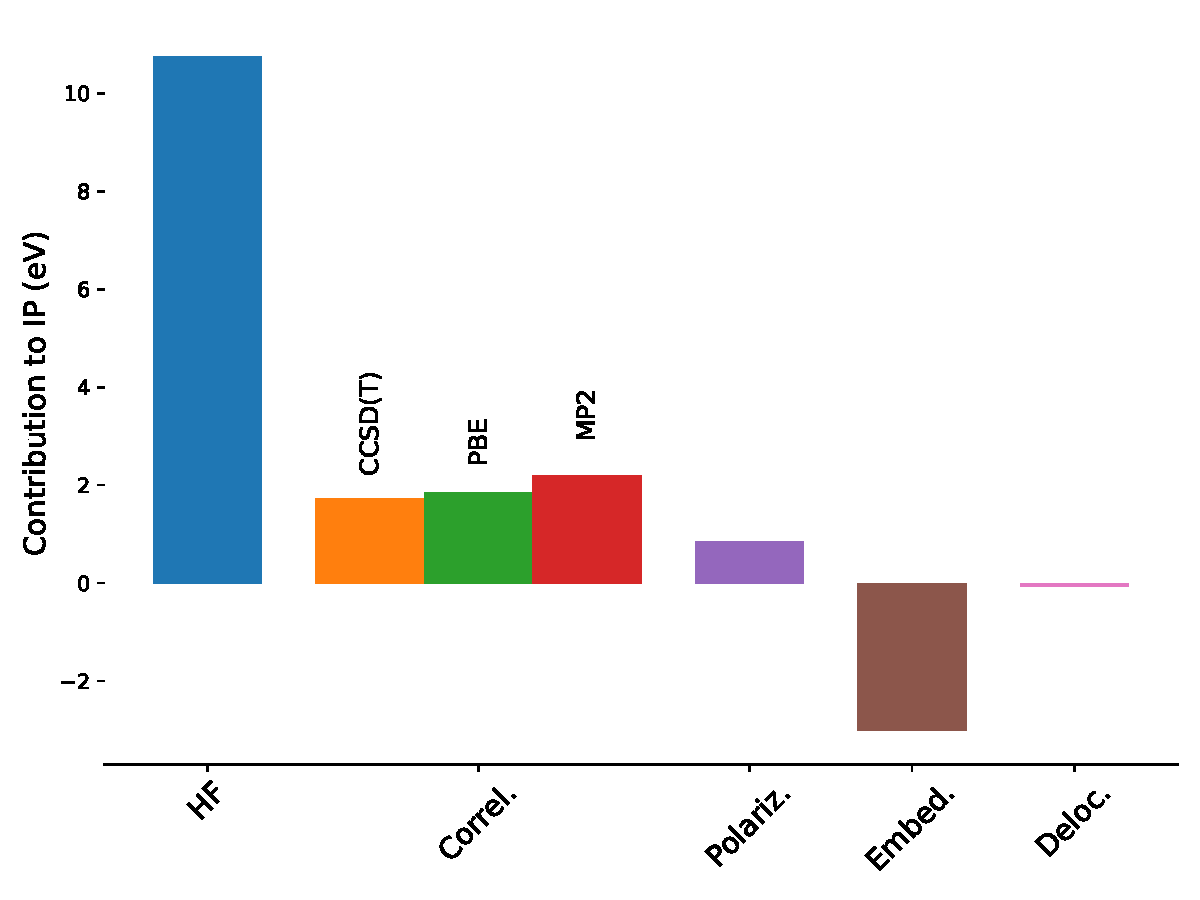
\includegraphics[width=\linewidth]{./images/contribution_liquidwater_PI}
    \caption{\label{cont_ip}Five contributions to the IP of water (see text). Their interplay highlights the complexity of the electronic processes occurring when water is ionized. \supercite{martinez2022ionization}}
\end{wrapfigure}

    The subsystem DFT description of the electronic structure in conjunction with the impurity model allowed us to break down the IP of liquid water  into five energy contributions \supercite{martinez2022ionization}:  {\bf (1)} Mean field (HF): the ionization energy of each water molecule computed at Hartree-Fock level; {\bf (2)} Correlation: electron correlation within each water molecule at the correlated wavefunction level as well as DFT; {\bf (3)} Embedding: Coulomb interactions between each water molecule and their environment augmented by effects of exchange, correlation and Pauli repulsion; {\bf (4)} Polarization: polarization of the environment electronic structure in response to the ionization of a nearby water molecule; and finally, {\bf (5)} Delocalization: the possibility that the spin density of the cation is delocalized over more than one water molecule. By averaging results from  128  snapshots of a 64-molecule model of liquid water (in periodic boundary conditions) \supercite{gaiduk2018electron}, the five contributions were calculated and are summarized in Figure \ref{cont_ip}. 

    The correlation contribution was calculated by DFT-embedded wavefunction methods such as CCSD(T) and MP2 as well as pure DFT functionals such as PBE and contributed by about 2 eV. The polarization of the electronic environment nearby an ionized water molecule contributes for about 0.84 eV while the embedding correction (i.e., the interaction with the environment) contributes negatively by 2.8 eV. Accounting for spin density delocalization over more than one water molecule contributed by a negligible amount. Such a granularity in the description of the ionization process is unprecedented and highlights the capabilities of the method developed by this collaboration. 	
	
\textbf{\large 2.\ Proposed work}
    
    With granted funding, the Chateaubriand fellowship will allow me to build upon the existing collaborative work to develop a comprehensive and accurate model of ionization {\bf and } core-electron excitation in molecular bulk systems. Leveraging the impurity model, I wish to combine the subsystem DFT and the real-time TDDFT embedding method based on the block-orthogonalized Manby-Miller embedding (BOMME) \supercite{ding2017embedded,koh2017accelerating} recently  developed by the Gomes group \supercite{De_Santis_2020,de2021environment} to extend my analysis of the ionization processes in water to also model X-Ray absorption and photoelectron spectroscopies (XAS, XPS)\supercite{fransson2016x}. Such spectroscopies  allow for a comprehensive characterization of the electronic state of species, such as their oxidation state, local symmetry, and coordination environment in gas, liquid, and solid phases\supercite{rehr2005progress,koningsberger1987x}. The BOMME approach is an alternative embedding method which focuses on embedding density matrices rather than electron densities. This has advantages in terms of accuracy of the method, but also carries some disadvantages interms of the increased computational complexity. My goal will be to combine the subsystem DFT (density embedding) for long-ranged interactions, and BOMME (density matrix embedding) for short-ranged interactions resulting in computational protocols that are as accurate as BOMME but with a computational complexity that is in between BOMME and subsystem DFT.

    The computational methods that I will develop together with Prof Gomes and Pavanello will have a strong impact in the computational materials science,  XPS and XAS communities. When metal complexes are solvated in water, it is known that hybridizations can occur between water and the metal \supercite{N_slund_2003}.  XAS and XPS of simply pure liquid water have also been a matter of intense study \supercite{fransson2016x} due to their ability to infer on water's hydrogen bond structure. There are multiple theoretical approaches for modeling XPS and XAS in molecular systems, such as transition potential (TP)-DFT  and TDDFT \supercite{triguero1998calculations}, excited-state core hole (XCH)\supercite{prendergast2006x}, GW (for valence electrons) \supercite{vinson2012theoretical,chen2010x}. To include the effect of the condensed phase, QM/MM techniques in conjunction with TDDFT have also been explored.\supercite{list2014lanczos} A detailed description of each approach is found in Ref.\ \cite{fransson2016x}. {\bf The most inconvenient shortcoming of the currently available methods is their computational cost which prevents them from ridding their simulations of the so-called finite size effects.} These have resulted in simulations which can only infer on the effect of the first solvation shell on the computation of the core-electron excitations\supercite{de2021environment}. 

    By incorporating Prof Gomes's BOMME approach in the eDFTpy\supercite{edftpy} {\bf open source} software of the Pavanello group in a hybrid density/density-matrix embedding scheme and its extension to the time domain for the computation of electronic excited states, I will focus on simulating the following 3 systems: (1) Liquid water\supercite{gaiduk2018electron} and Ice \supercite{bergmann2007nearest,zhovtobriukh2019x}, (2) monovalent cations (Li$^{+}$,Na$^{+}$,K$^{+}$,NH$_4^{+}$) ion-paired to carboxylate groups of acetate and glycine solvated in water \supercite{aziz2008cation}, and (3) transition metals solvated in water \supercite{N_slund_2003,zheng2018enabling}. Therefore the project will be divided into 3 stages: implementation, validation and application. I expect the three stages to take a similar amount of time, and to be largely complete by the end of the fellowship. I describe them in more details here below:
    \begin{itemize}
        \item {\bf Implementation} will require the development of several Python classes in the eDFTpy software to be able to accommodate the BOMME method from the Gomes lab. I will implement an object-oriented interface between approaches based on local orbitals (such as Psi4Numpy)  and ones based on plane waves (such as eDFTpy\supercite{edftpy} which is based in Quantum ESPRESSO \supercite{qe}). While the implementations will be ongoing by the time the fellowship starts, I expect them to continue upon my arrival to Lille.
        \item {\bf Validation} will take place at two levels: ground state and excited states. I will apply the method for the computation of simple interaction energies in molecular dimers which can be compared against benchmark values. Once this first stage is complete and the ground state implementation is validated, I will proceed to testing the code in its real-time TDDFT mode. This will allow me to model optical spectra of embedded (solvated) species as well as core-electron excitations. Validation for this stage will involve carefully documenting the effect of solvation on the computed  observables, including microsolvation which can be handled by supramolecular codes (i.e., no embedding).
        \item {\bf Application} will involve running ab-initio molecular dynamics simulations for sampling purposes using the developed software. In a second stage, I will sample a number of geometries form the dynamics trajectory to then compute ionization energies of valence electrons, core-electron excitations and optical spectra of the three systems mentioned before (liquid water, ice, and solvated cations). This will be a production-type calculations which will be carried out on the high-performance supercomputers in Lille as well as at Rutgers. 
    \end{itemize}


    I conclude mentioning that the implementations carried out as part of this project will be completely open source and available to anyone, stored in versioning servers (such as GitLab or GitHub). The software will not only impact this project, but because it is general and based on first principles, it can be applied to any molecular condensed phase system. Thus, a broad impact will accompany this project beyond the impact of the planned simulations, as we expect the collaborative efforts to also yield impactful and timely software.
\printbibliography

\end{document}
